%
% File naaclhlt2016.tex
%

\documentclass[11pt]{article}
\usepackage{style/naaclhlt2016}
\naaclfinalcopy
\def\naaclpaperid{234}

\usepackage{times}
\usepackage{url}
\usepackage{setspace}
\usepackage{latexsym}
\usepackage{CJKutf8}
\usepackage{multirow}
\usepackage{booktabs}
\usepackage{array}
\newcolumntype{L}[1]{>{\raggedright\let\newline\\\arraybackslash\hspace{0pt}}m{#1}}
\usepackage{ulem}
\usepackage{courier}
\usepackage{enumitem}
\usepackage{xcolor}
\usepackage[T1]{fontenc}
\normalem

\newcommand{\todo}[1]{({\bf TODO:} #1)}
\newcommand{\trans}{{Translationese}}
\newcommand{\inter}{{Interpretese}}
\newcommand{\jatext}[1]{\begin{CJK}{UTF8}{min}#1\end{CJK}}
\newcommand{\pos}[1]{{\small \texttt{#1}}}
\renewcommand{\S}{$\langle$S$\rangle$}
\renewcommand{\SS}{$\langle$SS$\rangle$}
\newcommand{\E}{$\langle$E$\rangle$}
\newcommand{\EE}{$\langle$EE$\rangle$}


\definecolor{darkblue}{rgb}{0.0,0.0,0.5}
\definecolor{darkpurple}{rgb}{0.4,0.0,0.4}
\definecolor{darkred}{rgb}{0.5,0.0,0.0}
\definecolor{darkgreen}{rgb}{0.0,0.5,0.0}

\newcommand{\summarized}[1]{\textcolor{darkred}{\uwave{#1}}}
\newcommand{\moregeneral}[1]{\emph{\textcolor{darkpurple}{#1}}}
\newcommand{\Segment}{\textcolor{darkgreen}{\langle\big\|\rangle}}
\newcommand{\passivized}[1]{\textcolor{darkblue}{\underline{#1}}}

\newcommand{\Gn}{\moregeneral{generalize}}
\newcommand{\Sg}{segment $\Segment$}
\newcommand{\Sm}{\summarized{summarize}}
\newcommand{\Ps}{\passivized{passivize}}
\newcommand{\Om}{(omit)}
\newcommand{\Source}[1]{{(S)\hspace{1ex}\jatext{#1}}}
\newcommand{\Trans}[1]{{(T)\hspace{1ex}#1}}
\newcommand{\Inter}[1]{{(I)\hspace{1ex}#1}}

\makeatletter
\newcommand{\@BIBLABEL}{\@emptybiblabel}
\newcommand{\@emptybiblabel}[1]{}
\makeatother
\usepackage{hyperref}

\naaclfinalcopy % Uncomment this line for the final submission

% To expand the titlebox for more authors, uncomment
% below and set accordingly.
% \addtolength\titlebox{.5in}

\frenchspacing
\newif\ifcomment\commentfalse

% Preamble file contains handy macros and most packages you might want to use.
% At the start are packages that conflict with various styles.  Don't add them
% in!  Just put it in your main TeX file instead.

% Do not put either of these (subfigure or subfloat) into the preamble
% - they clash.  Use them in the final LaTeX document
% \usepackage{subfigure}
% \suepackage{subfloat}

% Do not use times in the preamble!  It just causes problems with some
% publication chairs (e.g., ICML 2013).  If you want it, put it in your own
% document.
% \usepackage{times}


% Breaks ACM-SIG style
% \usepackage{titlesec}
% \usepackage{amsthm}
% \usepackage{nomencl}

% comment out the following line, as it conflicts with aistats2012.sty
%\usepackage{caption}


% Below should be safe
\usepackage{framed}
\usepackage{mdwlist}
\usepackage{latexsym}
\usepackage{xcolor}
\usepackage{nicefrac}
\usepackage{booktabs}
\usepackage{amsfonts}
\usepackage{bold-extra}
\usepackage{amsmath}
\usepackage{dsfont}
\usepackage{amssymb}
\usepackage{bm}
\usepackage{graphicx}
\usepackage{mathtools}
\usepackage{microtype}
\usepackage{multirow}
\usepackage{multicol}
%\usepackage{url}
\usepackage{latexsym,comment}

\newcommand{\breakalign}{\right. \nonumber \\ & \left. \hspace{2cm}}



\newcommand{\feat}[1]{{\small \texttt{#1}}}
\newcommand{\act}[1]{{\small \texttt{#1}}}
\newcommand{\ngram}[0]{$n$-gram}
\newcommand{\topic}[1]{\underline{#1}}
\newcommand{\gem}[1]{\mbox{\textsc{gem}}}
\newcommand{\abr}[1]{\textsc{#1}}
\newcommand{\camelabr}[2]{{\small #1}{\textsc{#2}}}
\newcommand{\abrcamel}[2]{{\textsc #1}{\small{#2}}}
\newcommand{\grammar}[1]{{\color{red} #1}}
\newcommand{\explain}[2]{\underbrace{#2}_{\mbox{\footnotesize{#1}}}}
\newcommand{\dir}[1]{\mbox{Dir}(#1)}
\newcommand{\bet}[1]{\mbox{Beta}(#1)}
\newcommand{\py}[1]{\mbox{\textsc{py}}(#1)}
\newcommand{\td}[2]{\mbox{\textsc{TreeDist}}_{#1} \left( #2 \right)}
\newcommand{\yield}[1]{\mbox{\textsc{Yield}} \left( #1 \right)}
\newcommand{\mult}[1]{\mbox{Mult}( #1)}
\newcommand{\wn}{\textsc{WordNet}}
\newcommand{\twentynews}{\textsc{20news}}
\newcommand{\g}{\, | \,}
\newcommand{\Gam}[1]{\Gamma \left( \textstyle #1 \right)}
\newcommand{\LG}[1]{\log \Gamma \left( \textstyle #1 \right)}
\newcommand{\Pois}[1]{\mbox{Poisson}(#1)}
\newcommand{\pcfg}[3]{#1_{#2 \rightarrow #3}}
\newcommand{\grule}[2]{#1 \rightarrow #2}
\newcommand{\kl}[2]{D_{\mbox{\textsc{KL}}} \left( #1 \,||\, #2 \right)}

\newcommand{\digambig}[1]{\Psi \left( #1 \right) }
\newcommand{\digam}[1]{\Psi \left( \textstyle #1 \right) }
\newcommand{\ddigam}[1]{\Psi' \left( \textstyle #1 \right) }

\DeclareMathOperator*{\argmax}{arg\,max}
\DeclareMathOperator*{\argmin}{arg\,min}
\newcommand{\bmat}[1]{\text{\textbf{#1}}}
\newcommand{\bvec}[1]{\boldsymbol{#1}}

\newcommand{\email}[1]{ {\small \href{mailto://#1}{\texttt{#1} }  }}
\newcommand{\emaillink}[2]{ {\small \href{mailto://#2}{\texttt{#1} }  }}

\newcommand{\ch}[1]{\begin{CJK*}{UTF8}{gbsn}#1\end{CJK*}}

\newcommand{\e}[2]{\mathbb{E}_{#1}\left[ #2 \right] }
\newcommand{\h}[2]{\mathbb{H}_{#1}\left[ #2 \right] }
\newcommand{\ind}[1]{\mathds{1}\left[ #1 \right] }
\newcommand{\ex}[1]{\mbox{exp}\left\{ #1\right\} }
\newcommand{\D}[2]{\frac{\partial #1}{\partial #2}}
\newcommand{\elbo}{\mathcal{L}}

\newcommand{\hidetext}[1]{}
\newcommand{\ignore}[1]{}

\newcommand{\todo}[1]{\textcolor{red}{{\bf TODO: #1}}}

\ifcomment
\newcommand{\pinaforecomment}[3]{\colorbox{#1}{\parbox{.8\linewidth}{#2: #3}}}
\else
\newcommand{\pinaforecomment}[3]{}
\fi

\newcommand{\jbgcomment}[1]{\pinaforecomment{red}{JBG}{#1}}
\newcommand{\mjpcomment}[1]{\pinaforecomment{blue}{MJP}{#1}}
\newcommand{\czcomment}[1]{\pinaforecomment{orange}{chen}{#1}}
\newcommand{\ffcomment}[1]{\pinaforecomment{red}{FF}{#1}}
\newcommand{\fpcomment}[1]{\pinaforecomment{green}{FP}{#1}}
\newcommand{\yhcomment}[1]{\pinaforecomment{green}{YH}{#1}}
\newcommand{\hhecomment}[1]{\pinaforecomment{blue}{HH}{#1}}
\newcommand{\tncomment}[1]{\pinaforecomment{blue}{TN}{#1}}
\newcommand{\mnicomment}[1]{\pinaforecomment{green}{Mohit}{#1}}
\newcommand{\prcomment}[1]{\pinaforecomment{lightblue}{Pedro}{#1}}
\newcommand{\fscomment}[1]{\pinaforecomment{orange}{Shi}{#1}}
\newcommand{\vmcomment}[1]{\pinaforecomment{yellow}{Varun}{#1}}
\newcommand{\rscomment}[1]{\pinaforecomment{yellow}{Richard}{#1}}
\newcommand{\jszcomment}[1]{\pinaforecomment{green}{JSG}{#1}}
\newcommand{\ascomment}[1]{\pinaforecomment{blue}{AS}{#1}}
\newcommand{\vecomment}[1]{\pinaforecomment{blue}{VE}{#1}}
\newcommand{\halcomment}[1]{\pinaforecomment{magenta!20}{Hal}{#1}}
\newcommand{\kgcomment}[1]{\pinaforecomment{blue}{Kim}{#1}}
\newcommand{\vancomment}[1]{\pinaforecomment{green}{VAN}{#1}}
\newcommand{\thangcomment}[1]{\pinaforecomment{green}{Thang}{#1}}
\newcommand{\alvincomment}[1]{\pinaforecomment{cyan}{Alvin}{#1}}
\newcommand{\reviewercomment}[1]{\pinaforecomment{blue}{Reviewer}{#1}}
\newcommand{\brscomment}[1]{\pinaforecomment{blue}{BRS}{#1}}
\newcommand{\psrcomment}[1]{\pinaforecomment{yellow}{PSR}{#1}}
\newcommand{\zkcomment}[1]{\pinaforecomment{cyan}{ZK}{#1}}
\newcommand{\swcomment}[1]{\pinaforecomment{yellow}{SW}{#1}}
\newcommand{\shaycomment}[1]{\pinaforecomment{yellow}{SBC}{#1}}
\newcommand{\jlundcomment}[1]{\pinaforecomment{cyan}{J}{#1}}
\newcommand{\kdscomment}[1]{\pinaforecomment{ceil}{KDS}{#1}}
\newcommand{\lkfcomment}[1]{\pinaforecomment{yellow}{LF}{#1}}
\newcommand{\yfcomment}[1]{\pinaforecomment{brown}{YF}{#1}}
\newcommand{\ewcomment}[1]{\pinaforecomment{lightblue}{Eric}{#1}}

\newcommand{\smalltt}[1]{ {\tt \small #1 }}
\newcommand{\smallurl}[1]{ \begin{tiny}\url{#1}\end{tiny}}
%\newcommand{\smallurl}[1]{ \begin{tiny} HIDDEN \end{tiny}}
\newenvironment{compactenum}{ \begin{enumerate*} \small }{ \end{enumerate*} }

\definecolor{lightblue}{HTML}{3cc7ea}
\definecolor{CUgold}{HTML}{CFB87C}
\definecolor{grey}{rgb}{0.95,0.95,0.95}
\definecolor{ceil}{rgb}{0.57, 0.63, 0.81}


% Datasets

\newcommand{\qb}[0]{Quizbowl}
\newcommand{\triviaqa}{\camelabr{Trivia}{qa}}
\newcommand{\qblink}{\abrcamel{qb}{Link}}
\newcommand{\qanta}{\textsc{qanta}}


\title{Interpretese vs. Translationese: \\ The Uniqueness of Human Strategies in Simultaneous Interpretation}

\author{He He \\
  Computer Science \\
  University of Maryland \\
  {\tt hhe@cs.umd.edu} \\\And
  Jordan Boyd-Graber \\
  Computer Science \\
  University of Colorado \\
{\tt Jordan.Boyd.Graber} \\
   {\tt @colorado.edu} \\ \And
  Hal {Daum\'e III} \\
  Computer Science and \abr{umiacs} \\
  University of Maryland \\
  {\tt hal@cs.umd.edu}}

\date{}

\begin{document}
\maketitle
\begin{abstract}
  Computational approaches to simultaneous interpretation are stymied
  by how little we know about the tactics human interpreters use. We
  produce a parallel corpus of translated and simultaneously
  interpreted text and study differences between them through a
  computational approach.  Our analysis reveals that human
  interpreters regularly apply several effective tactics to reduce
  translation latency, including sentence segmentation and
  passivization.  In addition to these unique, clever strategies, we
  show that limited human memory also causes other idiosyncratic
  properties of human interpretation such as generalization and
  omission of source content.
\end{abstract}

\section{Human Simultaneous Interpretation}
\label{sec:intro}

Although simultaneous interpretation has a key role in today's international
community,\footnote{Unlike consecutive interpretation (speakers stop
  after a complete thought and wait for the interpreter), simultaneous
  interpretation has the interpreter to translate \emph{while}
  listening to speakers.} it remains underexplored within machine
translation (\abr{mt}).  One key challenge is to achieve a good
quality/speed trade-off: deciding when, what, and how to translate.
In this study, \textbf{we take a data-driven, comparative approach and
  examine:} (i) What distinguishes simultaneously interpreted text
(\inter{}\footnote{Language produced in the
  process of translation is often considered a dialect of the target
  language: ``\trans{}''~\cite{translationese}.  Thus,
  ``\inter{}'' refers to interpreted language.})
from batch-translated text (\trans{})?  (ii) What strategies do human
interpreters use?

Most previous work focuses on qualitative
analysis~\cite{epic,erik11theory,shimizu14corpus} or pattern
counting~\cite{tohyama06lrec,att13speech}.  In contrast, we use a more
systematic approach based on feature selection and statistical tests.
In addition, most work ignores \emph{translated} text, making it hard
to isolate strategies applied by interpreters as opposed to general
strategies needed for any translation.  \newcite{shimizu14corpus} are
the first to take a comparative approach; however, they directly train
\abr{mt} systems on the interpretation corpus without explicitly
examining interpretation tactics.  While some techniques can be
learned implicitly, the model may also learn undesirable behavior such
as omission and simplification: byproducts of limited human working
memory (Section~\ref{sec:analysis}).

Prior work studies simultaneous interpretation of
Japanese$\leftrightarrow$English~\cite{tohyama06lrec,shimizu14corpus}
and Spanish$\leftrightarrow$English~\cite{att13speech}.  We focus on
Japanese$\leftrightarrow$English interpretation.  Since information
required by the target English sentence often comes late in the source
Japanese sentence (e.g., the verb, the noun being modified), we expect
it to reveal a richer set of tactics.\footnote{The tactics are
  consistent with those discovered on other language pairs in prior
  work, with additional ones specific to head-final to head-initial
  languages.}  Our contributions are three-fold.  First, we collect
new human translations for an existing simultaneous interpretation
corpus, which can benefit future comparative
research.\footnote{\url{https://github.com/hhexiy/interpretese}}
Second, we use classification and feature selection methods to examine
linguistic characteristics comparatively.  Third, we categorize human
interpretation strategies, including word reordering tactics and
summarization tactics.  Our results help linguists understand
simultaneous interpretation and help computer scientists build better
automatic interpretation systems.


\begin{table*}[t!]

\newcommand{\Tactic}[1]{\multirow{3}{*}{\begin{minipage}{0.1\textwidth}#1\end{minipage}}}
\newcounter{example}
\addtocounter{example}{1}
\newcommand{\id}{\arabic{example} \stepcounter{example}}
\centering
\singlespacing
{\footnotesize
\begin{tabular}{p{0.6ex}|L{0.8\textwidth}|l}
\toprule
& \multicolumn{1}{c|}{Source (S), translation (T) and interpretation (I) text} & Tactic \\
\midrule
\multirow{3}{*}{\id}&\Source{この日本語の待遇表現の特徴ですが英語から日本語へ直訳しただけでは表現できないといった特徴があります.}&\Tactic{\Gn\\\Sg\\\Om}\\
& \Trans{(One of) the characteristics of \moregeneral{honorific} Japanese is that it can not be \moregeneral{adequately} expressed when using a direct translation (from English to Japanese).} & \\
& \Inter{Now let me talk about the characteristic of the Japanese \moregeneral{polite} expressions. $\Segment$ And such such expressions can not be expressed \moregeneral{enough} just by translating directly.} & \\
\midrule
\multirow{3}{*}{\id}&\Source{で三番目の特徴としてはですねえ出来る限り自然な日本語の話言葉とてその出力をするといったような特徴があります.}&\Tactic{\Gn\\\Sm\\\Om}\\
& \Trans{Its third \moregeneral{characteristic} is that its output is, \summarized{as much as possible}, in the natural language of spoken (Japanese).} & \\
& \Inter{And the third \moregeneral{feature} is that the translation could be produced in a \summarized{very} natural spoken language.} & \\
\midrule
\multirow{3}{*}{\id}&\Source{まとめますと我々は派生文法という従来の学校文法とは違う文法を使った日本語解析を行っています.その結果従来よりも単純な解析が可能となっております.}&\Tactic{\Sg\\\Om}\\
& \Trans{In sum , we've conducted an analysis on the Japanese language , using a grammar different from school grammar, called derivational grammar. (As a result,) we were able to produce a simpler analysis (than the conventional method).} & \\
& \Inter{So, we are doing Japanese analysis based on derivational grammar, $\Segment$ which is different from school grammar, $\Segment$ which enables us to analyze in simple way.} & \\
\midrule
\multirow{3}{*}{\id}&\Source{つまり例えばこの表現一は認識できますが二から四は認識できない.}&\Tactic{\Gn\\\Ps\\\Sg}\\
& \Trans{\passivized{They might \moregeneral{recognize}} expression one but not \moregeneral{expressions} two to four.} & \\
& \Inter{The phrase number one only \passivized{is \moregeneral{accepted}} $\Segment$ and \moregeneral{phrases} two, three, four \passivized{were not \moregeneral{accepted}}.} & \\
\midrule
\multirow{3}{*}{\id}&\Source{以上のお話をまとめますと自然な発話というものを扱うことができる音声対話の方法ということを考案しました.}&\Tactic{\Gn\\\Ps\\\Sg}\\
& \Trans{In summary , \passivized{we have \moregeneral{devised}} a way for voice interaction systems \passivized{to handle} natural speech.} & \\
& \Inter{And this is the summary of what I have so far stated. The spontaneous speech \passivized{can be dealt with} by the speech dialog method $\Segment$ and that method \passivized{was \moregeneral{proposed}}.} & \\
\bottomrule
\end{tabular}
}

\caption{Examples of tactics used by interpreters
to cope with divergent word
  orders, limited working memory, and the pressure to produce low-latency translations.  
  We show the source input (S), translated sentences (T), and interpreted sentences (I).
  The tactics are listed in the rightmost column and marked in
  the text:  more general translations are highlighted in
  \moregeneral{italics}; $\Segment$ marks where new clauses or sentences are created;
  and passivized verbs in translation \passivized{are underlined}.
  Information appearing in translation but omitted in interpretation are in (parentheses).
  Summarized expressions and their corresponding expression in translation are \summarized{underlined by wavy lines}.}
  
  
\label{tab:examples}

\vspace{-1em}
\end{table*}
\section{Distinguishing \trans{} and \inter{}}
\label{sec:distinguish}

In this section, we discuss strategies used in \inter{}, which we
detect automatically in the next section.  Our hypothesis is that
tactics used by interpreters roughly fall in two non-exclusive
categories: (i) \emph{delay minimization}, to enable prompt
translation by arranging target words in an order similar to the
source; (ii) \emph{memory footprint minimization}, to avoid
overloading working memory by reducing communicated information.








\paragraph{Segmentation}

Interpreters often break source sentences into multiple smaller
sentences~\cite{erik11theory,shimizu13iwslt}, a process we call segmentation.
This is different from what is commonly used in speech translation
systems~\cite{fujita13timing,oda14segmentation}, where translations of segments
are directly concatenated.  Instead, humans try to incorporate new information
into the precedent partial translation, e.g., using ``which is'' to put it in a
clause (Table~\ref{tab:examples}, Example~3), or creating a new sentence joined
by conjunctions (Table~\ref{tab:examples}, Example~5).

\paragraph{Passivization}

Passivization is useful for interpreting from head-final
languages (e.g., Japanese, German) to head-initial languages (e.g., English,
French)~\cite{he15rewrite}.  Because the verb is needed early in the target sentence but only
appears at the end of the source sentence, an obvious strategy is to wait for the final
verb.  However, if the interpreter uses passive voice, they can start translating
immediately and append the verb at the end (Table~\ref{tab:examples},
Examples~3--4).  During passivization, the subject is often omitted when obvious
from context.


















\paragraph{Generalization}

\newcite{erik11theory} and \newcite{raja00strategy} observe that interpreters
focus on delivering the gist of a sentence rather than duplicating the
nuanced meaning of each word.  More frequent words are chosen as their
retrieval time is faster~\cite{dell92access,cuetos06access} (e.g.,
``honorific'' versus ``polite'' in Table~\ref{tab:examples},
Example~1).  Although \newcite{volansky13feats} show that
generalization happens in translation too, it is likely more frequent
in \inter{} given the severe time constraints.

\paragraph{Summarization}

Faced with overwhelming information, interpreters need efficient ways to
encode meaning.  Less important words, or even a whole sentence can drop,
especially when the interpreter falls behind the speaker.  In
Table~\ref{tab:examples}, Example~2, the literal translation ``as much as
possible'' is reduced to ``very'', and the adjective ``Japanese'' is omitted.

\begin{figure}
\centering
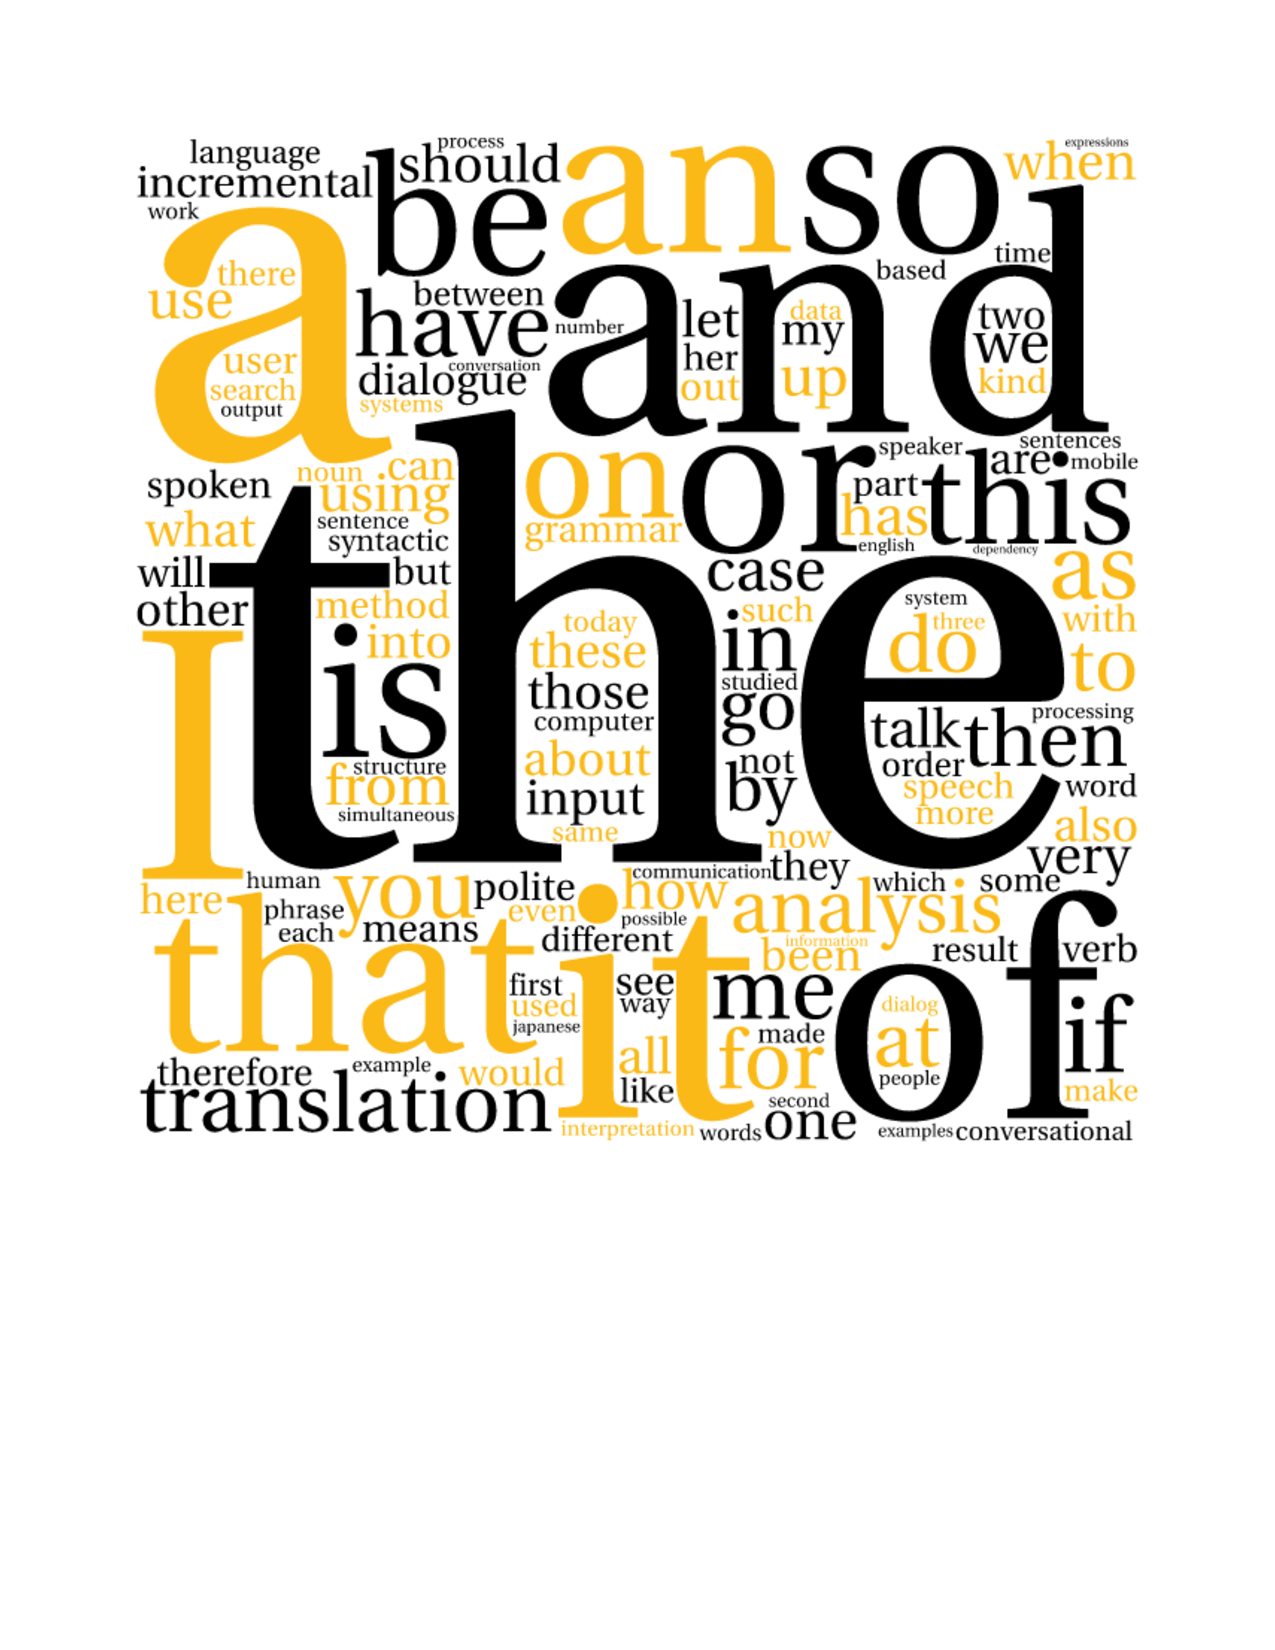
\includegraphics[width=0.7\linewidth]{2016_naacl_interpretese/figures/wordle.pdf}
\caption{A word cloud visualization of \inter{} (black) and \trans{} (gold).}
\label{fig:wordle}
\end{figure}



\paragraph{}

Before we study these characteristics quantitatively in the next section, we
visualize \inter{} and \trans{} by a word cloud in Figure~\ref{fig:wordle}.  The
size of each word is proportional to the difference between its frequencies in
\inter{} and \trans{} (Section~\ref{sec:experiments}).  The word color indicates
whether it is more frequent in \inter{} (blue) or \trans{} (red).  ``the'' is
over-represented in \inter{}, a phenomenon also occurs in \trans{} v.s. the
original text~\cite{eetemadi14feats}.  More conjunction words (e.g., ``and'',
``so'', ``or'', ``then'') are used in \inter{}, likely for segmentation, whereas
``that'' is more frequent in \trans{}---a sign of clauses.  In addition, the
pronoun ``I'' occurs more often in \trans{} while ``be'' and ``is'' occur more
often in \inter{}, which is consistent with our passivization hypothesis.

\section{Classification of \trans{} and \inter{}}
\label{sec:experiments}

We investigate the difference between \trans{} and \inter{} by
creating a text classifier to distinguish between them and then
examining the most useful features. We train our classifier on a
bilingual Japanese-English corpus of spoken monologues and their
simultaneous interpretations~\cite{ciair}.  To obtain a three-way
parallel corpus of aligned translation, interpretation, and their
shared source text, we first align the interpreted sentences to source
sentences by dynamic programming following
\newcite{champollion}.\footnote{Sentences are defined by sentence
  boundaries marked in the corpus, thus coherence is preserved during
  alignment.} This step results in 1684 pairs of text chunks, with 33
tokens per chunk on average.  We then collect human translations from
Gengo\footnote{\url{http://gengo.com} (``standard'' quality).} for
each source text chunk (one translator per monologue).  The original
corpus has four interpretors per monologue. We use all available
interpretation by copying the translation of a text chunk for its
additional interpretation.

\subsection{Discriminative Features}
\label{sec:classification_results}

We use logistic regression as our classifier.  Its job is to tell, given a chunk
of English text, which translation produced it.  We add $\ell_1$ regularization
to select the non-zero features that best distinguish \inter{} from \trans{}.
We use three different sets of features: (1) \textbf{\abr{POS}:} $n$-gram
features of \abr{POS} tags (up to trigram);~\footnote{We prepend \pos{\S{}} and
  append \pos{\E{}} to all sentences.}  (2) \textbf{\abr{LEX}:} word unigrams;
(3) \textbf{\abr{LING}:} features reflecting linguistic hypothese
(Section~\ref{sec:distinguish}), most are counts of indicator functions
normalized by length of the chunk (Appendix~\ref{sec:features}).

The top linguistic features listed in Table~\ref{tab:feat} are consistent with
our hypotheses.  The most prominent ones---also revealed by \abr{pos} and
\abr{lex}---are the segmentation features, including counts of conjunction words
(\feat{CC}), content words (nouns, verbs, adjectives, and adverbs) that appear
more than once (\feat{repeated}), demonstratives (\feat{demo}) such as
\emph{this, that, these, those}, segmented sentences (\feat{sent}), and proper
nouns (\feat{NNP}).  More conjunction words and more sentences in a text chunk
are signs of segmentation.  Repeated words and the frequent use of
demonstratives come from transforming clauses to independent sentences.
Next are the passivization features, indicating more passivized verbs
(\feat{passive}) and fewer pronouns (\feat{pronoun}) in \inter{}.





The lack of pronouns may be results of either subject omission during
passivization or general omission.  The last group are the vocabulary features,
showing fewer numbers of stem types, token types, and content words in \inter{},
evidence of word generalization.  In addition, a smaller number of content words
suggests that interpreters may use more function words to manipulate the sentence
structure.

\subsection{Classification Results}













\begin{table*}[t!]
\centering
\singlespacing
\renewcommand{\arraystretch}{0.8}
{\footnotesize
\begin{tabular}{c|ccc|c|cc|cc|c}
\toprule
Sample & inv-all & inv-verb & inv-noun & segment & pass-t & pass-st & omit & insert & word freq \\
\midrule
$H_a$ & \multicolumn{3}{c|}{$\mu_I < \mu_T$} & $\mu_I > \mu_T$ & \multicolumn{2}{c|}{$\mu_I > \mu_T$} & \multicolumn{2}{c|}{$\mu_I > \mu_T$} & $\mu_I > \mu_T$ \\
$t$-stat & -1.55 & \bf{-3.81} & \bf{-2.13} & \bf{4.21} & \bf{5.67} & 1.41 & \bf{16.16} & \bf{10.66} & \bf{7.88} \\
$p$-value & .12 & $<$.001 & .03 & $<$.001 & $<$.001 & .16 & $<$.001 & $<$.001 & $<$.001\\
\bottomrule
\end{tabular}
}
\caption{Two-sample $t$-tests for \inter{} and \trans{}.  The test
  statistics are bolded when we reject $H_0$ at the 0.05 significance
  level (two-tailed).








}
\label{tab:ttest}
\end{table*}

Recall that our goal is to understand \inter{}, not to classify
\inter{} and \trans{}; however, the ten-fold cross validation accuracy
of \abr{LING}, \abr{POS}, \abr{LEX} are 0.66, 0.85, and 0.94.
\abr{LEX} and \abr{POS} yield high accuracy as some features are
overfitting, e.g., in this dataset, most interpreters used ``parsing''
for ``\jatext{構文解析}'' while the translator used ``syntactic
analysis''.  Therefore, they do not reveal much about the
characteristics of \inter{} except for frequent use of ``and'' and
\pos{CC}, which indicates segmentation.  Similarly,
\newcite{volansky13feats} and \newcite{eetemadi14feats} also find
lexical features very effective but not generalizable for detecting
Translationese and exclude them from analysis.  One reason for the
relatively low accuracy of \abr{ling} may be inconsistent use of
strategies among humans (Section~\ref{sec:analysis}).

\begin{table}[t!]
\centering
\singlespacing
\renewcommand{\arraystretch}{0.8}
\newcommand{\+}{+}
\renewcommand{\-}{\textendash}
\renewcommand{\pos}[1]{{\footnotesize \texttt{#1}}}
{\footnotesize
\begin{tabular}{l@{\hspace{0.7ex}}p{2ex}|l@{\hspace{0.7ex}}p{2ex}|l@{\hspace{0.7ex}}p{2ex}}
\toprule
\abr{ling} & & \abr{pos} & & \abr{lex} & \\
\midrule
\textsf{CC} & \+ & \pos{\S{} CC} & \+ & And & \+ \\
\textsf{repeated} & \+ & \pos{. CC} & \+ & parsing & \+ \\
\textsf{demo} & \+ & \pos{\S{} CC IN} & \+ & gradual & \- \\
\textsf{sent} & \+ & \pos{NN CC PR} & \+ & syntax & \- \\
\textsf{passive} & \+ & \pos{\S{} CC DT} & \+ & keyboard & \+ \\
\textsf{pronoun} & \- & \pos{CC RB DT} & \+ & attitudinal & \- \\
\textsf{NNP} & \+ & \pos{, RB DT} & \+ & text & \- \\
\textsf{stem type} & \- & \pos{. CC DT} & \+ & adhoc & \+ \\
\textsf{tok type} & \- & \pos{NN FW NN} & \+ & construction & \- \\
\textsf{content} & \- & \pos{NN CC RB} & \- & Furthermore & \- \\
\bottomrule
\end{tabular}
}
\caption{Top 10 highest-weighted features in each model.
The sign shows whether it is indicative of \inter{} (+) or \trans{} (\textendash).
}
\label{tab:feat}
\end{table}

\section{Strategy Analysis}
\label{sec:analysis}





















To better understand under what situations these tactics are used, we
apply two-sample $t$-tests to compare the following quantities between
\inter{} and \trans{}: (1) number of inversions (non-monotonic
translations) on all source tokens ({inv-all}), verbs ({inv-verb}) and
nouns ({inv-noun}); (2) number of segmented sentences; (3) number of
natural passivization ({pass-st}), meaning copying a passive
construction in the source sentence into the target sentence, and
intentional passivization ({pass-t}), meaning introducing
passivization into the target sentence when the source sentence is in
active voice; (4) number of omitted words on the source side and
inserted words on the target side;\footnote{The number
  of unaligned words in the source or target.}
(5) average word frequency given by Microsoft Web $n$-gram---higher
means more
common.\footnote{\url{http://weblm.research.microsoft.com/}} For all
pairs of samples, the null hypothesis $H_0$ is that the means on
\inter{} and \trans{} are equal; the alternative hypotheses and
results are in Table~\ref{tab:ttest}.

As expected, segmentation and intentional passivization happen more
often during interpretation.  \inter{} has fewer inversions, especially
for verbs; reducing word order difference is
important for delay minimization.  Since there are two to four
different interpretations for each lecture, we further analyze how
consistent humans are on these decisions.  All interpreters agree on
segmentation 73.7\% of the time, while the agreement on passivization
is only 57.1\%---passivization is an acquired skill; not all
interpreters use it when it can speed interpretation.

The tests also confirm our hypotheses on generalization and omission.
However, these tactics are not inherent to the task of simultaneous
interpretation.  Instead, they are a byproduct of humans' limited
working memory.  Computers can load much larger resources into memory
and weigh quality of different translations in an instant, thus
potentially rendering the speaker's message more accurately.
Therefore, directly learning from corpus of human interpretation may
lead to suboptimal results~\cite{shimizu14corpus}.

\section{Conclusion}
\label{sec:conclusion}

While we describe how \trans{} and \inter{} are different and
characterize \emph{how} they differ, the contribution of our work is
not just examining an interesting, important dialect.  Our work
provides opportunities to improve conventional simultaneous MT systems
by exploiting and modeling human tactics.  \newcite{he15rewrite} use
hand-crafted rules to decrease latency; our data-driven approach could
yield additional strategies for improving \abr{mt} systems.  Another
strategy---given the scarcity and artifacts of interpretation
corpus---is to select references that present delay-minimizing
features of \inter{} from translation
corpus~\cite{axelrod11selection}.  Another future direction is to
investigate cognitive inference~\cite{inference-in-interpretation},
which is useful for semantic/syntactic prediction during
interpretation~\cite{grissom14simtrans,oda15acl}.

\appendix


\section{Feature Extraction}
\label{sec:features}

We use the Berkeley aligner~\cite{berkeleyaligner} for word alignment,
the Stanford \abr{pos} tagger~\cite{stanford-tagger} to tag English
sentences, and Kuromoji~\footnote{\url{http://www.atilika.org/}} to
tokenize, lemmatize and tag Japanese sentences.  Below we describe the
features in detail.

\noindent
\textbf{Inversion:} Let $\{A_i\}$ be the set of indexes of target
words to which each source word $w_i$ is aligned.  We count $A_i$ and
$A_j$ ($i < j$) as an inverted pair if $\max(A_i) > \min(A_j)$.  This
means that we have to wait until the $j$th word to translate the $i$th
word.

\noindent
\textbf{Segmentation:}
We use the \texttt{punkt} sentence segmenter~\cite{kiss06segmenter}
from \abr{NLTK} to detect sentences in a text chunk.
















\noindent
\textbf{Passivization:}
We compute the number of passive verbs normalized by the total number
of verbs.  We detect passive voice in English by matching the
following regular expression: a \emph{be} verb (be, are, is, was, were
etc.) followed by zero to four non-verb words and one verb in its past
participle form.  We detect passive voice in Japanese by checking that
the dictionary form of a verb has the suffix ``\jatext{れる}''.









\noindent
\textbf{Vocabulary}
  To measure variety, we use $V_t/N$ and $V_s/N$, where $V_t$ and
  $V_s$ are counts of distinct tokens and stems, and $N$ is the total
  number of tokens.  To measure complexity, we use word length, number
  of syllables per word, approximated by vowel sequences; and unigram
  and bigram frequency from Microsoft Web $N$-gram.

\noindent
\textbf{Summarization}
We use the sentence compression ratio, sentence length, number of
omitted source words, approximated by counts of unaligned words, and
number of content words.

\section*{Acknowledgments}

We thank CIAIR (Nagoya University, Japan) for providing the interpretation data which
formed the foundation of this research.
We also thank Alvin Grissom~II, Naho Orita and the reviewers for their insightful comments.
This work was supported by
\abr{nsf} grant \abr{iis}-1320538.  Boyd-Graber is also partially
supported by \abr{nsf} grants \abr{ccf}-1409287 and
\abr{ncse}-1422492. Any opinions, findings,
conclusions, or recommendations expressed here are those of the
authors and do not necessarily reflect the view of the sponsor.

%\clearpage

\bibliographystyle{style/naaclhlt2016}
\bibliography{bib/journal-full,bib/jbg,bib/hhe}

\end{document}
